\documentclass{standalone}
\usepackage{tikz}
\usepackage{kpfonts}
\usepackage{xcolor-solarized}
\usetikzlibrary{decorations.pathmorphing}
\usetikzlibrary{positioning}
\usetikzlibrary{shapes.misc}
\usetikzlibrary{shapes.geometric}
\usetikzlibrary{shapes.symbols}
\usetikzlibrary{arrows}
\usetikzlibrary{fit}
\usetikzlibrary{backgrounds}

\begin{document}
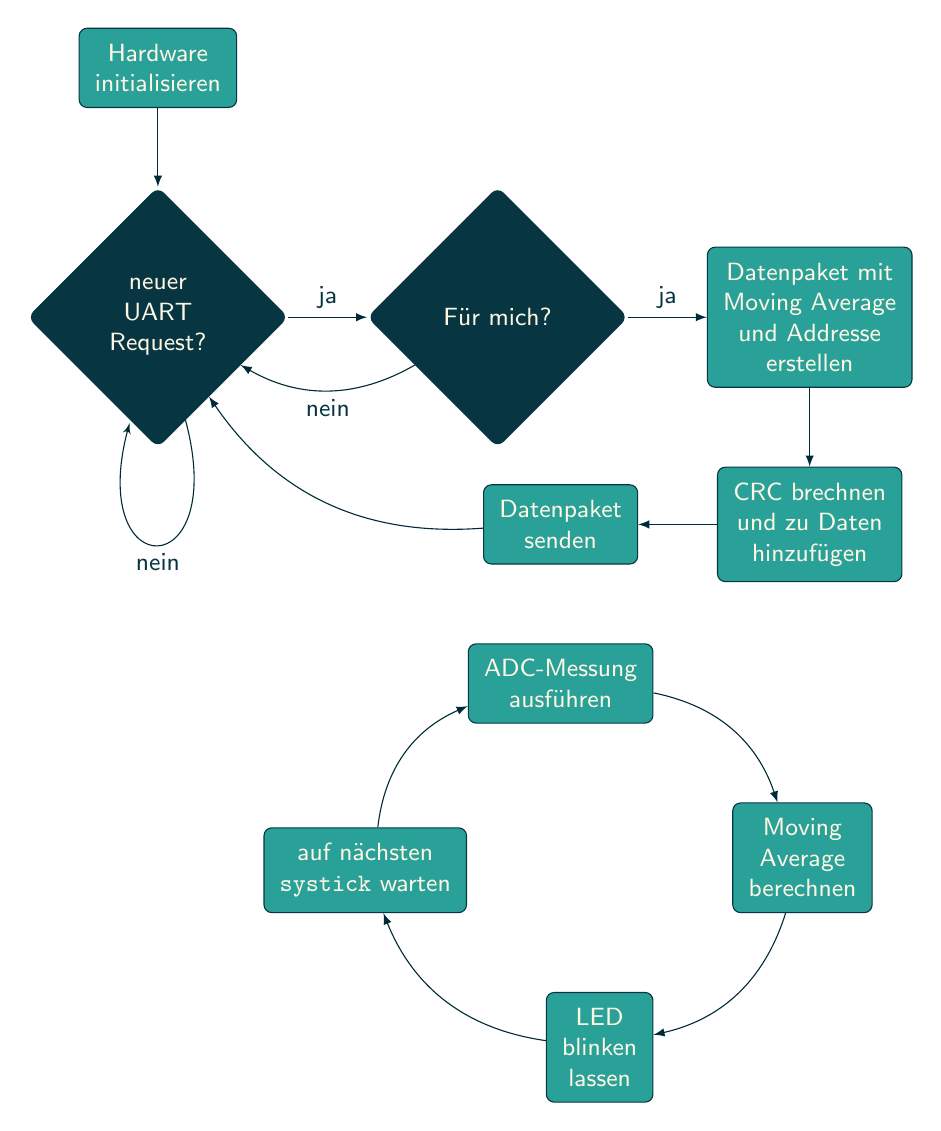
\begin{tikzpicture}[%
        align=center,
        text=solarized-base02,
        draw=solarized-base02,
    ]
    \small
    \sffamily

    \begin{scope}[
        every node/.style = draw,
        terminal/.append style={
            rounded rectangle,
            fill=solarized-violet,
            text=solarized-base3,
            inner sep=2mm,
        }, % data packages
        sign/.style={
            inner sep=2mm,
            rounded corners=1mm,
            fill=solarized-magenta,
            text=solarized-base3,
        },         % custom signal style
        circ/.style={
            inner sep=2mm,
            rounded corners=1mm,
            double,
            fill=solarized-base02,
            draw=solarized-base02,
            text=solarized-base2,
        }, % circuitry
        proc/.style={
            inner sep=2mm,
            rounded corners=1mm,
            fill=solarized-cyan,
            text=solarized-base3,
        },       % process/activity
        dec/.style={
            inner sep=2mm,
            rounded corners=1mm,
            fill=solarized-base02,
            text=solarized-base3,
        },       % decision/activity
        stor/.style={
            fill=cyan!30
        },         % storage
        dbtable/.style={
            text=solarized-base3,
            draw=solarized-base3,
            rounded corners=1mm,
            inner sep=2mm,
        } % database tables
    ]
        \node (newUART) [
            dec,
            align=center,
            diamond,
            minimum width=33mm,
            minimum height=33mm,
        ] at (0,0) {neuer\\UART\\Request?};
        \node (init) [
            proc,
            above=of newUART,
            align=center,
        ] {Hardware\\initialisieren};
        \node (forMe) [
            dec,
            align=center,
            diamond,
            right=of newUART,
            minimum width=33mm,
            minimum height=33mm,
        ] {F\"ur mich?};
        \node (package) [
            proc,
            right=of forMe,
            align=center,
        ] {Datenpaket mit\\Moving Average\\ und Addresse\\erstellen};
        \node (crc) [
            proc,
            below=of package,
            align=center,
        ] {CRC brechnen\\und zu Daten\\hinzuf\"ugen};
        \node (send) [
            proc,
            left=of crc,
            align=center,
        ] {Datenpaket\\senden};
        \node (getADC) [
            proc,
            below=of send,
            align=center,
        ] {ADC-Messung\\ausf\"uhren};
        \node (movAvg) [
            proc,
            below right=of getADC,
            align=center,
        ] {Moving\\Average\\berechnen};
        \node (LED) [
            proc,
            below left=of movAvg,
            align=center,
        ] {LED\\blinken\\lassen};
        \node (systick) [
            proc,
            above left=of LED,
            align=center,
        ] {auf n\"achsten\\\texttt{systick} warten};
    \end{scope}

    \begin{scope}[
            rounded corners,
            every path/.append style={draw=solarized-base03,},
            >=latex',
    ]
        \draw[-latex] (init) -- (newUART);
        \draw[-latex] (newUART) -- node[midway,anchor=south] {ja} (forMe);
        \draw[-latex] (forMe) -- node[midway,anchor=south] {ja} (package);
        \draw[-latex] (package) -- (crc);
        \draw[-latex] (crc) -- (send);
        \draw[-latex] (forMe) edge[bend left] node[midway,anchor=north] {nein} (newUART);
        \draw[-latex] (send) edge[bend left] (newUART);
        \draw (newUART) edge[loop below]  node {nein} (newUART);

        \draw[-latex] (getADC) edge[bend left] (movAvg);
        \draw[-latex] (movAvg) edge[bend left] (LED);
        \draw[-latex] (LED) edge[bend left] (systick);
        \draw[-latex] (systick) edge[bend left] (getADC);

    \end{scope}

\end{tikzpicture}
\end{document}
